\chapter{IMPLEMENTATION} \label{c5}
\justifying

\section{Overview}

This chapter describes the implementation of the Sign Language Interpreter system, covering the development environment, core algorithms, and user interface approach.

\vspace{1em}
\section{Development Environment}

The system runs on Python 3.8+ with standard laptop hardware and webcam. Key dependencies include MediaPipe for hand landmark detection, OpenCV for video capture, scikit-learn for the Random Forest classifier, Streamlit for the web UI, and pyttsx3 for text-to-speech. No GPU is required as Random Forest inference is lightweight.

\vspace{1em}
\section{Core Modules}

The system consists of seven Python modules implementing the processing pipeline.

The video capture module initializes the webcam at 640x480 resolution, applies horizontal flip for mirror effect, and converts BGR to RGB color space. The hand detection module uses MediaPipe to extract 21 landmarks per hand with min\_detection\_confidence of 0.7 and min\_tracking\_confidence of 0.5.

The feature extraction module normalizes all landmarks relative to the wrist position (landmark 0) to create hand-pose-invariant features, flattening the 21 points to a 42-dimensional vector:

\begin{equation}
x_i' = x_i - x_{wrist}, \quad y_i' = y_i - y_{wrist} \quad \text{for } i = 0, ..., 20
\end{equation}

The representative code snippet:
\begin{lstlisting}[language=Python]
def normalize_landmarks(landmarks):
    wrist = landmarks[0]
    normalized = []
    for lm in landmarks:
        normalized.append([lm[0] - wrist[0], lm[1] - wrist[1]])
    return normalized

def extract_features(landmarks):
    normalized = normalize_landmarks(landmarks)
    features = []
    for lm in normalized:
        features.extend(lm)
    return np.array(features).reshape(1, -1)
\end{lstlisting}


\begin{figure}[H]
\centering
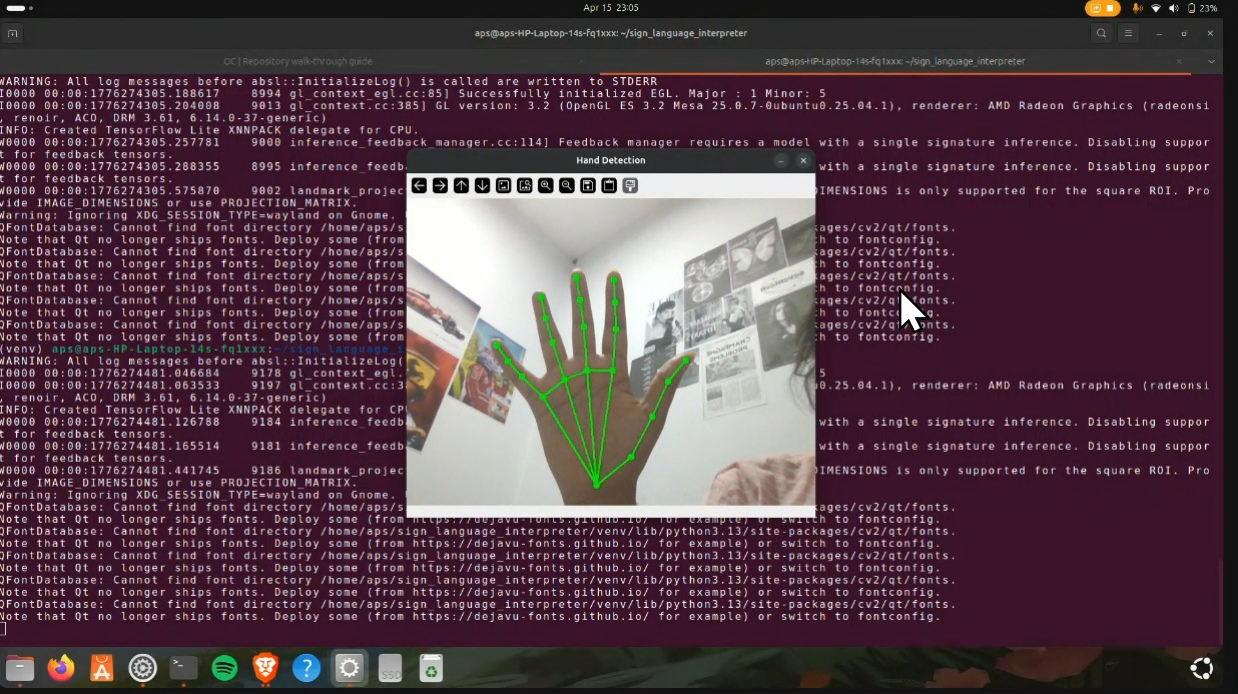
\includegraphics[width=0.7\textwidth]{images/hand_detect.jpeg}
\caption{Hand Landmark Detection Output}
\label{c5:fig1}
\end{figure}

The Random Forest classifier uses 200 trees with max depth 15, trained on 6,500+ samples, achieving 94.1\% test accuracy. The stability checker requires 15 consecutive frames with confidence above 0.85 before accepting a prediction. The text processing module buffers letters into words, with special gestures (index+middle fingers down for space, fist with thumb for delete) triggering word completion and character deletion. Text-to-speech uses pyttsx3 at 150 WPM with 0.9 volume.

\vspace{1em}
\section{User Interface}

Two UI options are provided: a Streamlit-based web interface offering interactive widgets with real-time webcam feed, prediction display, confidence indicators, and control buttons; and a Flask-based server with MJPEG streaming for lightweight deployments. Both render hand landmark overlays on the video feed and display the word buffer.

The inference pipeline executes sequentially: capture frame, detect hand, extract features, classify, check stability, update text buffer, display output, repeat at 30 FPS. Data collection runs the same pipeline with 250 samples per letter saved to CSV format.

\vspace{1em}
\section{Summary}

This chapter covered the implementation: seven modular Python components, wrist-centered feature normalization, Random Forest classification with 94.1\% accuracy, stability checking, text-to-speech integration, and optional Streamlit or Flask web UIs.